\todo[inline]{Diagramm}

\begin{figure}[H]
\centering
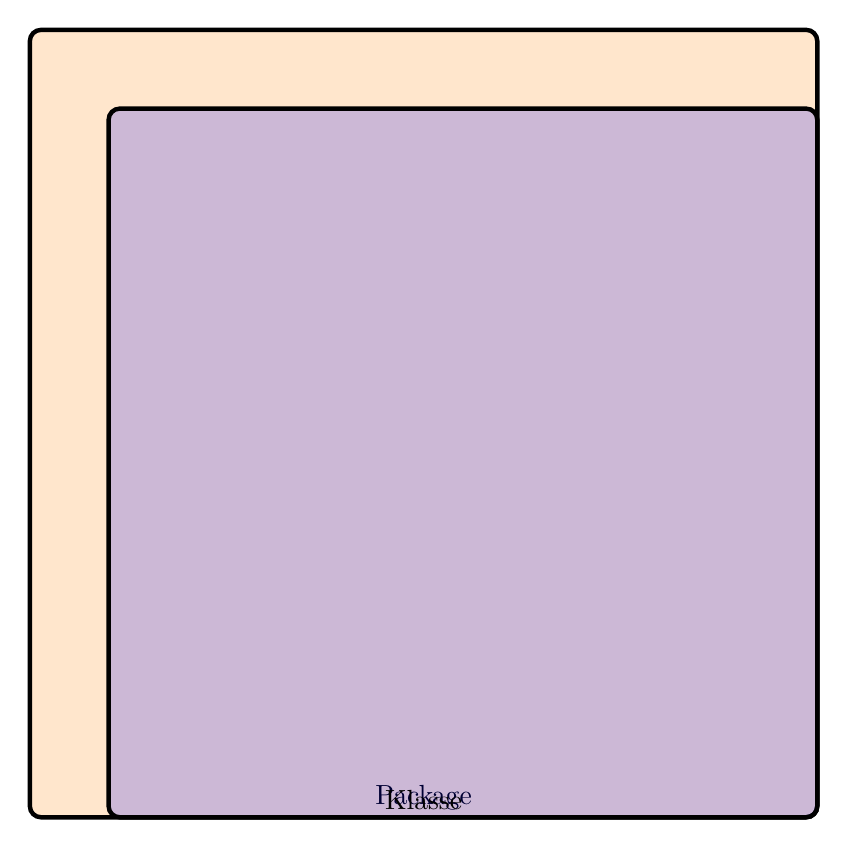
\begin{tikzpicture}

\node (packageRect) [rectangle, draw, rounded corners, ultra thick, draw=black, fill=orange, fill opacity=0.2, draw opacity=1, text opacity=1, anchor=south, minimum width=100mm, minimum height=100mm] at (0mm,0mm) {};
\node[above] (packageRect.center) {Package};

\node (classRect) [rectangle, draw, rounded corners, ultra thick, draw=black, fill=blue, fill opacity=0.2, draw opacity=1, text opacity=1, anchor=south, minimum width=90mm, minimum height=90mm] at (5mm,0mm) {};
\node[above] (classRect.center) {Klasse};

\end{tikzpicture}
\caption{Strukturelle Bestandteile eines Java-Programms}
\label{javaStructureDiagram}
\end{figure}

